\subsection{Protocol Overview}
\subsubsection{Roles}
A protocol run involves three roles: Alice, Bob, and a server. In this description, Alice wants to send an encrypted message to Bob. Bob is the party that may be offline at that time and wishes to enable other parties to derive a shared secret with it, through a set of public information Bob publishes. The server is responsible for 1. storing the public information published by Bob, and 2. storing messages for offline parties till they are fetched. The server is not trusted, however, it is assumed to be resilient against DoS. % more details.
\subsubsection{Keys}
\gls{x3dh} utilizes Elliptic Curve asymmetric key pairs. All keys used in a protocol run must all be derived from the same curve, either $X25519$ or $X448$. Each role has to have a set of keys to run the protocol. Table \ref{tab:x3dhkeys} lists the public keys required for each role. Note that for each public key, there exists a corresponding private key at its owner.

\begin{table}
	\centering
	\begin{tabular}{|c|c|c|}
		
		\hline
		\rowcolor[rgb]{ .745, .804, .843}
		Owning Role 			 & Notation							 & Description 			 \\ \hline\hline
		\multirow{2}{*}{Alice} 	 & \acrshort{ik}\textsubscript{A} 	 & Long-term \acrlong{ik} \\
		& EK\textsubscript{A} 	   		 & Ephemeral Key 		 \\\hline
		\multirow{3}{*}{Bob} 	 & \acrshort{ik}\textsubscript{B} 	 & \acrlong{ik} 		 \\
		& SPK\textsubscript{B} 			 & Signed Prekey 		 \\
		& OPK\textsubscript{B} 	 		 & one-time Prekey 		 \\ \hline
		
	\end{tabular}
	\caption{\gls{x3dh} keys.}
	\label{tab:x3dhkeys}
\end{table}

\begin{itemize}
	\item \textit{Identity keys}: They are long-term public keys known by their corresponding parties before the protocol run.
	\item \textit{Ephemeral Keys}: This type of key pair is freshly generated within the protocol run.
	\item \textit{Signed Prekey}: This key pair is generated and signed by its owner. The prekey is signed using the private identity key. The life time of this key pair is shorter than that of the identity key pairs as it is updated periodically by its owner. The corresponding role owns only one signed prekey at a time.
	\item \textit{One-time Prekey}: The corresponding role generates multiple one-time prekey. Each is can be used for only one protocol run. The responsible party is supposed to supply the these keys as they should not run out. In case there are not any keys left, the protocol can run, however without one of the \gls{dh} operations as explained in section 2.3.
\end{itemize}

\subsubsection{A Protocol Run}
%\subsubsubsection{Registration phase} 
At first, the protocol starts with a registration phase. Initially, The party acting in the role of Bob publishes to server the public information required to run the protocol with it by any party acting as Alice. Bob publishes his $ \gls{ik}_{B} $, $ SPK_{B} $, Bob's prekey signature, and a set of $ OPK_{B} $.

\par
%\subsubsubsection{The initial message}
Next, the inline party sends the initiates the protocol by sending the first message. First of all, Alice fetches a \textit{prekey bundle} from the server to contact Bob. This bundle contains:
\begin{itemize}
	%	\setlength\itemsep{-0.3em}
	\item Bob's Identity key $ \gls{ik}_{B} $.
	\item Bob's signed prekey $ SPK_{B} $.
	\item Bob's prekey signature.
	\item If exists, a one-time prekey $ OPK_{B} $. The server deletes the $ OPK_{B} $ sent to Alice.
\end{itemize}

Before proceeding, Alice verifies the prekey signature and quits the protocol if the verification fails.
At this point, Alice has enough information from Bob to deduce a shared secret. Alice generates her Ephemeral key pair $ EK_{A} $. With the set of available keys, Alice performs three \gls{dh} operations which are extended to four if a $ OPK_{B} $ is available. Figure \ref{fig:x3dh} presents the relation between the keys.

\begin{itemize}	
	\item $ DH1 = DH(\gls{ik}_{A_{p}} \footnote{\textit{p} indicates the private key of the key pair.}, SPK_{B}) $
	\item $ DH2 = DH(EK_{A_{p}}, \gls{ik}_{B}) $
	\item $ DH3 = DH(EK_{A_{p}}, SPK_{B}) $
	\item \textcolor{darkgray}{$ DH4 = DH(EK_{A_{p}}, OPK_{B}) $}
\end{itemize}

\begin{figure}[htbp]
	\centering
	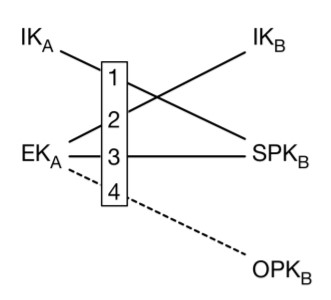
\includegraphics[width=0.4\linewidth]{images/X3dh}
	\caption{\gls{x3dh} operations \cite{x3dh}.}
	\label{fig:x3dh}
\end{figure}

The \gls{dh} outputs are fed into a \gls{kdf} to generate the shared secret $ SK $. Next, Alice deletes her $ EK_{A_{p}}$ and all \gls{dh} outputs for forward secrecy. At this moment, Alice is ready to send the initial message with the content encrypted using $ SK $. The initial message from Alice to Bob has to have enough information for Bob to generate the same $ SK $.
The initial message contains:
\begin{itemize}
	%	\setlength\itemsep {-0.3em}
	\item $ \gls{ik}_{A} $
	\item $ EK_{A} $
	\item Identifiers of Bob's prekeys used by Alice
	\item An initial ciphertext. The ciphertext can be used as an initial message for a post-X3DH communication protocol, e.g. Double Ratchet algorithm.
\end{itemize}

%\subsubsubsection{Bob's $ SK $ Derivation}
Upon receiving the initial message, Bob attempts to derive the $ SK $.
Using the key identifiers sent by Alice, Bob loads the private keys corresponding to the public keys Alice used. In combination with the keys $ \gls{ik}_{A} $ and $ EK_{A} $ Alice sent, Bob can compute the same $ SK $ by doing the three (or four) \gls{dh} operations.
\par
Next, Bob attempts to decrypt the ciphertext. If the message is successfully decrypted to the expected format, e.g. the format of the first message of the post-X3DH protocol, then the protocol run was successful. Otherwise, Bob aborts the protocol and discards the $ SK $.

\subsubsection{Security Considerations}
%\subsubsubsection{Authentication}
Authentication is essential for both parties to guarantee the identity of who they are communicating with. Thus, Alice and Bob must authenticate the keys $ \gls{ik}_{A} $ and $ \gls{ik}_{B} $. However, the protocol specification does not discuss authentication methods.
\par
%\subsubsubsection{Protocol Replay}
The one-time prekey used in the fourth and optional \gls{dh} calculation is for protection against replay attacks as they ensure freshness of the protocol run. Absence of a one-time prekey could lead a replayed message to be accepted by Bob believing that Alice had sent it in the current protocol run.
\par
%\subsubsubsection{Server Trust}
A server can be a cause of attacks if malicious. It can carry out a Denial of Service attack if it refuses to forward the messages. It can deliberately not distribute one-time prekeys, exposing the protocol to replay attacks. Also, one party can drain all the one-time prekeys, if the server is not attentive to such action, leading to replay attacks.
